\documentclass[unicode,11pt,a4paper,oneside,numbers=endperiod,openany]{scrartcl}

\usepackage{xcolor}
\usepackage{listings}
\usepackage{amsmath}

\lstnewenvironment{grayverbatim}{%
  \lstset{backgroundcolor=\color{gray!10}, % Adjust the shade of gray as desired
          frame=single,
          framerule=0pt,
          basicstyle=\ttfamily,
          breaklines=true,
          columns=fullflexible}
}{}

\lstnewenvironment{cppverbatim}{%
  \lstset{language=C++, % Set the language to C++
          backgroundcolor=\color{gray!10}, % Adjust the shade of gray as desired
          frame=single,
          framerule=0pt,
          basicstyle=\ttfamily,
          keywordstyle=\color{blue}, % Set the color for keywords
          commentstyle=\color{green!50!black}, % Set the color for comments
          stringstyle=\color{red}, % Set the color for strings
          breaklines=true,
          showstringspaces=false, % Don't show spaces within strings
          columns=fullflexible}
}{}

\usepackage{ifthen}
\usepackage[utf8]{inputenc}
\usepackage{graphics}
\usepackage{graphicx}
\usepackage{hyperref}

\pagestyle{plain}
\voffset -5mm
\oddsidemargin  0mm
\evensidemargin -11mm
\marginparwidth 2cm
\marginparsep 0pt
\topmargin 0mm
\headheight 0pt
\headsep 0pt
\topskip 0pt        
\textheight 255mm
\textwidth 165mm

\newcommand{\duedate} {}
\newcommand{\setduedate}[1]{%
\renewcommand\duedate {Due date:~ #1}}
\newcommand\isassignment {false}
\newcommand{\setassignment}{\renewcommand\isassignment {true}}
\newcommand{\ifassignment}[1]{\ifthenelse{\boolean{\isassignment}}{#1}{}}
\newcommand{\ifnotassignment}[1]{\ifthenelse{\boolean{\isassignment}}{}{#1}}

\newcommand{\assignmentpolicy}{
\begin{table}[h]
\begin{center}
\scalebox{0.8} {%
\begin{tabular}{|p{0.02cm}p{16cm}|}
\hline
&\\
\multicolumn{2}{|c|}{\Large\textbf{HPC Lab for CSE 2024 ---  Submission Instructions}}\\
\multicolumn{2}{|c|}{\large\textbf{(Please, notice that following instructions are mandatory: }}\\
\multicolumn{2}{|c|}{\large\textbf{submissions that don't comply with, won't be considered)}}\\
&\\
\textbullet & Assignments must be submitted to \href{https://moodle-app2.let.ethz.ch/course/view.php?id=22516}{Moodle} (i.e. in electronic format).\\
\textbullet & Provide both executable package and sources (e.g. C/C++ files, Matlab). 
If you are using libraries, please add them in the file. Sources must be organized in directories called:\\
\multicolumn{2}{|c|}{\textit{Project\_number\_lastname\_firstname}}\\
& and  the  file must be called:\\
\multicolumn{2}{|c|}{\textit{project\_number\_lastname\_firstname.zip}}\\
\multicolumn{2}{|c|}{\textit{project\_number\_lastname\_firstname.pdf}}\\
\textbullet &  The TAs will grade your project by reviewing your project write-up, and looking at the implementation 
                 you attempted, and benchmarking your code's performance.\\

\textbullet & You are allowed to discuss all questions with anyone you like; however: (i) your submission must list anyone you discussed problems with and (ii) you must write up your submission independently.\\
\hline
\end{tabular}
}
\end{center}
\end{table}
}
\newcommand{\punkte}[1]{\hspace{1ex}\emph{\mdseries\hfill(#1~\ifcase#1{Points}\or{Points}\else{Points}\fi)}}


\newcommand\serieheader[6]{
\thispagestyle{empty}%
\begin{flushleft}

\includegraphics[width=0.4\textwidth]{ETHlogo_13}
\end{flushleft}
  \noindent%
  {\large\ignorespaces{\textbf{#1}}\hspace{\fill}\ignorespaces{ \textbf{#2}}}\\ \\%
  {\large\ignorespaces #3 \hspace{\fill}\ignorespaces #4}\\
  \noindent%
  \bigskip
  \hrule\par\bigskip\noindent%
  \bigskip {\ignorespaces {\Large{\textbf{#5}}}
  \hspace{\fill}\ignorespaces \large \ifthenelse{\boolean{\isassignment}}{\duedate}{#6}}
  \hrule\par\bigskip\noindent%  \linebreak
 }

\makeatletter
\def\enumerateMod{\ifnum \@enumdepth >3 \@toodeep\else
      \advance\@enumdepth \@ne
      \edef\@enumctr{enum\romannumeral\the\@enumdepth}\list
      {\csname label\@enumctr\endcsname}{\usecounter
        {\@enumctr}%%%? the following differs from "enumerate"
	\topsep0pt%
	\partopsep0pt%
	\itemsep0pt%
	\def\makelabel##1{\hss\llap{##1}}}\fi}
\let\endenumerateMod =\endlist
\makeatother




\usepackage{textcomp}






\begin{document}


\setassignment
\setduedate{Monday 29 April 2024, 23:59 (midnight).}

\serieheader{High-Performance Computing Lab for CSE}{2024}
            {Student: CARLA JUDITH LOPEZ ZURITA}
            {Discussed with: ALITZEL ADRIANA MACIAS INFANTE}{Solution for Project 4}{}
\newline

\assignmentpolicy

\section{Ring sum using MPI [10 Points]}
The idea of this task is to implement a ring sum using MPI. The ring sum is a
simple algorithm to compute the sum of all elements in an array. To avoid any
deadlocks, I decided to use the
MPI\_Sendrecv function to send and receive the data.
The MPI\_Sendrecv is specially useful when you want to send and receive data
between two processes. The function is non-blocking, which means that the
function returns immediately after the data is sent and received. This avoids
any potential deadlocks.
The destination and source ranks are calculated as follows:
\begin{cppverbatim}
int rank_dest, rank_source;
rank_source = (rank + size - 1)
rank_dest = (rank + 1)
\end{cppverbatim}
The messages are chosen to be the sum of the current rank and the previous
received message, which is done repeatedly over the number of ranks so to
calculate the whole sum. The code block shows the logic used;
\begin{cppverbatim}
int out_msg, in_msg;
if (i == 0)
{
    out_msg = rank;
}
sum = sum + in_msg;
out_msg = in_msg;
\end{cppverbatim}
Finally, he code block below aims to give an idea of the function parameters, data types and
assigned values (it is not meant to represent the actual syntax used in the
implementation):
\begin{cppverbatim}
MPI_Sendrecv(
    const void *sendbuf = &out_msg,
    int sendcount = 1,
    MPI_Datatype sendtype = MPI_INT,
    int dest = rank_dest,
    int sendtag = 0,
    void *recvbuf = &in_msg,
    int recvcount = 1,
    MPI_Datatype recvtype = MPI_INT,
    int source = rank_source,
    int recvtag = 0,
    MPI_Comm comm = MPI_COMM_WORLD,
    MPI_Status *status = &status
)
\end{cppverbatim}
The code was tested with 5 processes and the result is 10.

\section{Cartesian domain decomposition and ghost cells exchange [20 Points]}
The objective of this task is to implement a 2D Cartesian domain decomposition
and exchange ghost cells between neighboring processes. The idea is to divide a
2D grid into smaller subgrids, where each subgrid is assigned to a process. The
borders are assigned the value of the neighboring process. 
To implement this, I used the MPI\_Cart\_create and MPI\_Cart\_shift functions
to create a 2D Cartesian topology and to get the neighboring processes.
To communicate the column ghost cells, I created a new MPI datatype using the
MPI\_Type\_vector function using the domain and subdomain sizes, defined as follows:
\begin{cppverbatim}
MPI_Type_vector(SUBDOMAIN, 1, DOMAINSIZE, MPI_DOUBLE, &data_ghost_col);
MPI_Type_commit(&data_ghost_col);
\end{cppverbatim}
Afterwards, I used the MPI\_Send and MPI\_Recv function to communicate the
messages because it is sufficient and easier to implement. This implementation seemed to work well for the given test case,
although it may not be thread safe for other cases. For the given test case, the
buffer was enough to store the data and the communication was successful.
An example of the implementation regarding the first row and interaction with
the top block is added below:
\begin{cppverbatim}
// SEND
//  to top
MPI_Send(&data[first_row_index], 1, data_ghost_row, rank_top, tag, MPI_COMM_WORLD);

// RECEIVE
// from top
MPI_Recv(&data[first_row_index], 1, data_ghost_row, rank_top, tag, MPI_COMM_WORLD, &status);
\end{cppverbatim}
Some auxiliary variables were used to store the ranks of the desired cells (rows
and columns).
The complete implementation can be found in the attached code. The code was
tested with a $6x6$ matrix, $8x8$ considering ghost cells. We report the boundary exchange on rank 9.
\begin{grayverbatim}
9.0  5.0  5.0  5.0  5.0  5.0  5.0 9.0
8.0  9.0  9.0  9.0  9.0  9.0  9.0 10.0
8.0  9.0  9.0  9.0  9.0  9.0  9.0 10.0
8.0  9.0  9.0  9.0  9.0  9.0  9.0 10.0
8.0  9.0  9.0  9.0  9.0  9.0  9.0 10.0
8.0  9.0  9.0  9.0  9.0  9.0  9.0 10.0
8.0  9.0  9.0  9.0  9.0  9.0  9.0 10.0
9.0 13.0 13.0 13.0 13.0 13.0 13.0 9.0
\end{grayverbatim}

\section{Parallelizing the Mandelbrot set using MPI [30 Points]}
The goal of this task is to parallelize the computation of the Mandelbrot set
using OpenMP. We use the base code of the previous project and modify it to use
MPI. The idea is to divide the image into smaller subimages and assign each
subimage to a process. This should be done automatically, without any manual
input. This is done using \textit{Partition} and \textit{Domain} structs, which
contain information such as index
of the pixels, size, and coordinated of the subimages.
These data structures are based on the functions MPI\_Dims\_create, MPI\_Cart\_create,
MPI\_Cart\_coords to create a 2D Cartesian topology and to get the coordinates,
similar to the previous task. 
In this implemtation, we area also using the MPI\_Send and MPI\_Recv functions
to communicate the data between the processes. The data is sent and received a
contiguos vector of pixels. Each subimage is compued in separate processes and
sent to the root process, which is responsible for storing and creating the final image.
Figure \ref{fig:mandelbrot} shows the result of the computation of the
Mandelbrot set using 4096x4096 pixels distributeed over 16 processes. 
\begin{figure}[h!]
    \centering
    
\includegraphics[width=0.5\textwidth]{../mandel/mandel.png}
    \caption{Mandelbrot set}
    \label{fig:mandelbrot}
\end{figure}
We can see that the image reproduces the correct result, as we obtianed in a previous project. 
The performance
of the parallel Mandelbrot set using this implementation is shown in Figure \ref{fig:mandelbrot_parallel}.
It reflects how the work is distributed among the processes and the time taken
by each. 
\begin{figure}[h!]
    \centering
    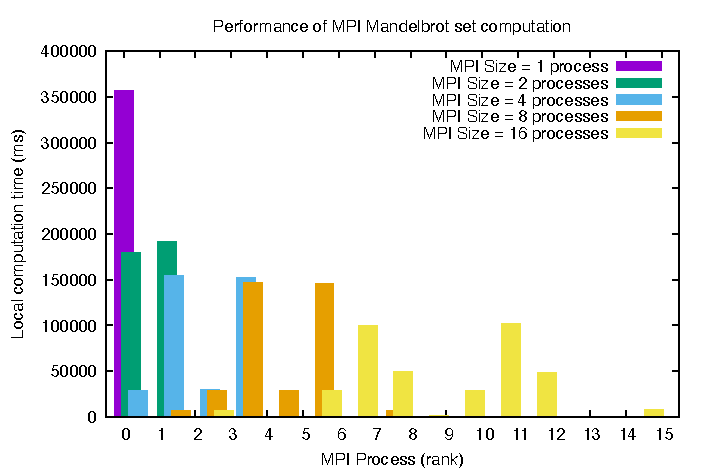
\includegraphics[width=0.8\textwidth]{../mandel/perf.pdf}
    \caption{Parallel Mandelbrot set}
    \label{fig:mandelbrot_parallel}
\end{figure}
We can see that as the number of processes increases, the time taken per process
to compute their part of the image decreases in comparison to the single
processor implementation but not equally among all processes. This is because
the work of the Mandelbrot set is not evenly distributed spacially, that is to
say, some parts of the image are more complex to compute than others. The graph
reflects that the partition between the processes is not optimal, as some of the
processes do not reduce the time significantly as the number of processes
increases. A more efficient partitioning algorithm could be implemented to solve
this issue, but this would require previous knowledge of the desired solution.
Another approach could be to use a dynamic partitioning algorithm, which would
distribute the work among the processes according to the complexity of the
computation.


\section{Parallel matrix-vector multiplication and the power method
[40 Points]}

The goal of this task is to complete a code trying to parallelize the
matrix-vector multiplication and the power method using MPI. This was achieved
using MPI\_Bcast and MPI\_Allgatherv functions. The idea is to broadcast the
original vector solution $y$ of size $n$ and then gather the results from all processes
which were computed in $y_{local}$, of size $nrows_{local}$. The implementation of this specific part is
shown below:
\begin{cppverbatim}
MPI_Bcast(y, n, MPI_DOUBLE, 0, MPI_COMM_WORLD);
...
MPI_Allgatherv(y_local, nrows_local, MPI_DOUBLE, y, recvcounts, displs, MPI_DOUBLE, MPI_COMM_WORLD);
\end{cppverbatim}

The variable \textit{recvcounts} is an array that contains the number of
elements to be received from each process. The \textit{displs} array contains
the displacement of the data to be received. The code was tested with a matrix
of $10,000\times 10,000$, with a maximum of $3,000$ iterations, using test
number $3$, which resulted in a eigenvalue of $9998.059$. The strong and weak
scaling of the matrix-vector multiplication and the power method are shown in
Figures \ref{fig:strong_scaling} and \ref{fig:weak_scaling}, respectively. 
The scaling was done using one core as well as multiple cores.
The
time used as reference was the parallel implementation with 1 process. The
reported value is the mean of fifty runs. We can see that the strong scaling
presents a more than linear speedup, which is odd. This could be attributted to
the overhead of the communication between the processes when not comparing against
the naive implementation. For some reason, this is not present in the run over
multiple cores. 

\begin{figure}[h!]
    \centering
    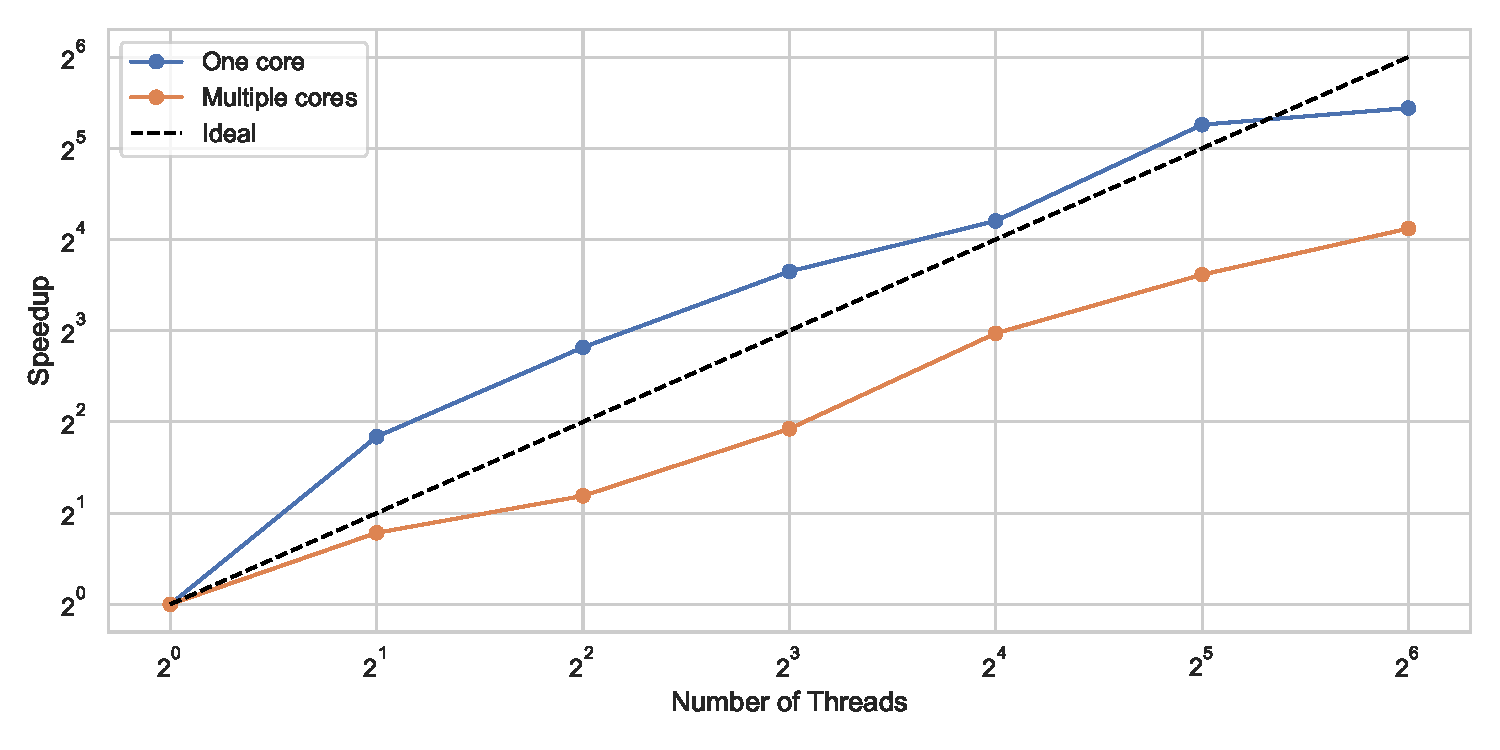
\includegraphics[width=0.8\textwidth]{../powermethod/strong_scaling_plot.pdf}
    \caption{Strong scaling of the matrix-vector multiplication and the power method.}
    \label{fig:strong_scaling}
\end{figure}
The weak scaling shows a good performance in the low number of processes, but
then it starts to decrease. This can be attributed to the overhead of the
communication. 
\begin{figure}[h!]
    \centering
    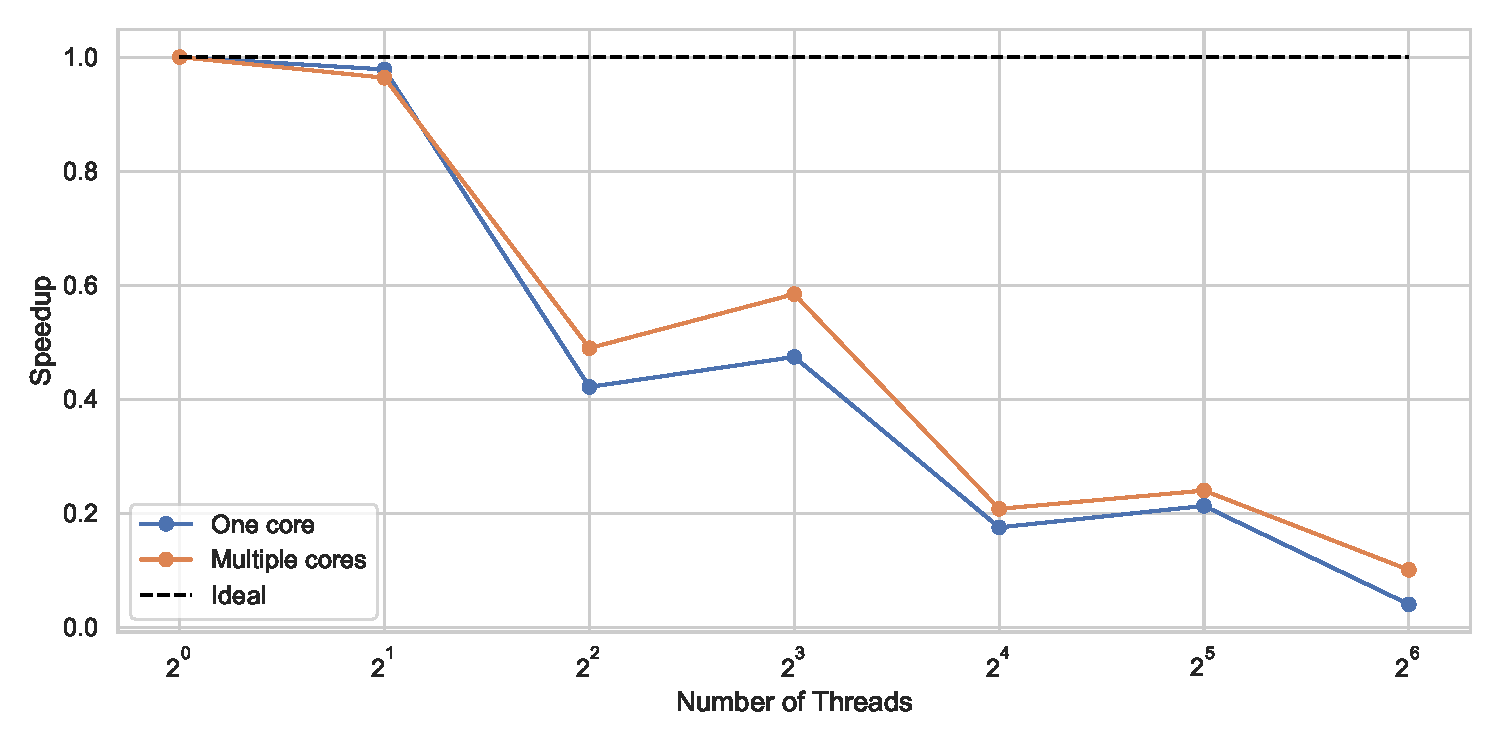
\includegraphics[width=0.8\textwidth]{../powermethod/weak_scaling_plot.pdf}
    \caption{Weak scaling of the matrix-vector multiplication and the power method.}
    \label{fig:weak_scaling}
\end{figure}
Contrary to the strong scaling, the weak scaling shows similar performance for
both runs over one and multiple cores.

\end{document}
